\chapter{Návrh systému}
\label{kap_navrh_systemu}
V předchozích dvou kapitolách byla rozebrána teoretická část problému. V následující kapitole shrneme požadavky z teorie vyplývající, které je nutno zakomponovat do
výsledného systému. Nejprve bude schématicky vyjádřena obecná funkcionalita systému, která se následně bude rozebírat detailněji.

\section{Teoretické požadavky}
Nároky na systém, které vyplývají z teorie můžeme rozdělit do třech částí - implementace SNMP protokolu, implementace navrženého XML protokolu a propojení těchto dvou protokolů dohromady.

Hlavním požadavkem, který vyplývá i ze zadání práce, je vytvořit modulární systém, který bude nejenom spojovat současné verze protokolů, ale bude počítat i s potenciálním rozšířením do
budoucna. Obecné schéma navrhovaného systému zobrazuje obrázek \ref{obr_an_obecne_schema}. 

\begin{figure}[htp]
	\begin{center}
		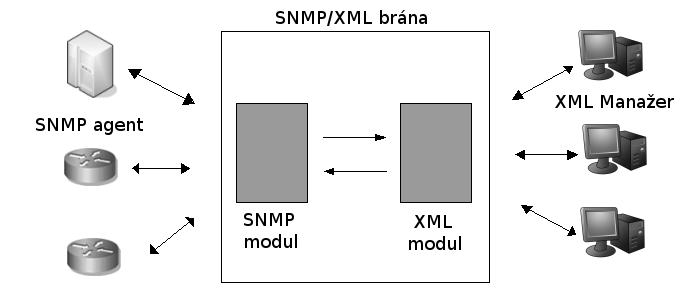
\includegraphics[width=15cm]{obrazky/03_obecne_schema.png}
		\caption{Schéma navrhovahého systému}
		\label{obr_an_obecne_schema}
	\end{center}
\end{figure}

Zde je vidět, že oba dva protokolové moduly jsou na sobě nezávislé a jejich interakce spočívá v předávání si zpráv. Nyní přejděme k detailnějším požadavkům na výše zmíněné části systému.

V rámci \textit{SNMP protokolu} je požadováno
\begin{itemize}
	\item implementace komunikačních struktur protokolů SNMPv1 a SNMPv2
	\item převzetí bezpečnostního schématu z tohoto protokolu
\end{itemize}

\textit{XML orientovaná část programu } má za úkol
\begin{itemize}
	\item implementovat komunikační struktury navrženého protokolu
	\item navrhnout efektivní správu XML struktur v paměti
	\item poskytnout XML manažerům transparentní získání dat z monitorovaných zařízení
	\item mapovat rozšířenou množinu funkcí v rámci XML protokolu do SNMP
	\item s manažery komunikovat pouze přes HTTP/HTTPS protokol
\end{itemize}

Spojením protokolů je myšlen přechod od databázových struktur jednoho protokolu k druhému. V našem případě je to transformace SNMP MIB do XML, jak bylo vysvětleno v kapitole \ref{kap_xml}.

\subsection{XML}
%TODO
%zminit XML strom pri zpracovani zprav a zaroven vyuziti XPath, XQuery
%definovat presne tu strukturu XML stromu!!!
%zpravy
%komunikacni protokol
%zabezpeceni


\subsection{SNMP}
%TODO
%zpravy
%bezpecnost



\section{Struktura programu}
%TODO
%krok za krokem vyjadrit, jak bude program nabihat a bezet
%config file navrhnout
%build XML tree  (transform from MIB)
%atd atd (viz struktura_programu v analyze)
%DISKUSE na SOAP vs. demon
%DISKUSE ohledne sdileni nodu v xml stromu
